\chapter{The heritage of IXPE}
\label{chap:chapter3}

Imaging X-ray Polarimetry Explorer (IXPE) \cite{weisskopf2021} is a mission launched in 2021 by NASA and ASI to study polarization of bright X-ray sources, capable of doing imaging, spectroscopy and timing measurements as well. IXPE is the first mission ever entirely dedicated to soft X-ray polarimetry, and it has a sensitivity more than an order of magnitude higher than Bragg crystal polarimeters used on board of older missions.

This large increase in sensitivity was achievable thanks to the innovations brought by the Gas Pixel Detectors (GPD) \cite{baldini2021}, the class of detectors used on board of IXPE. GPD use photoelectric effect to infer the degree of polarization of a source, in particular they exploit the dependence of the emission angle of the photoelectron on the photon polarization. By collecting enough photons it is possible to measure the polarization of the source by studying the distribution of events as a function of the emission angle.

As of 2026, IXPE is still carrying on observational campaigns, even though the nominal lifetime is only two years. In five years of operations IXPE has observed and measured the polarization of about 100 sources. 

IXPE consists of three identical and independent X-ray telescopes. Each telescope has its grazing incidence mirrors with Wolter-1 configuration and a focal length of 4 m. The mirrors are made of 24 concentric and nested foils of nickel and cobalt, and the layout is optimized for high sensitivity in the range 2--8 keV.

\begin{figure}[!b]
    \centering
    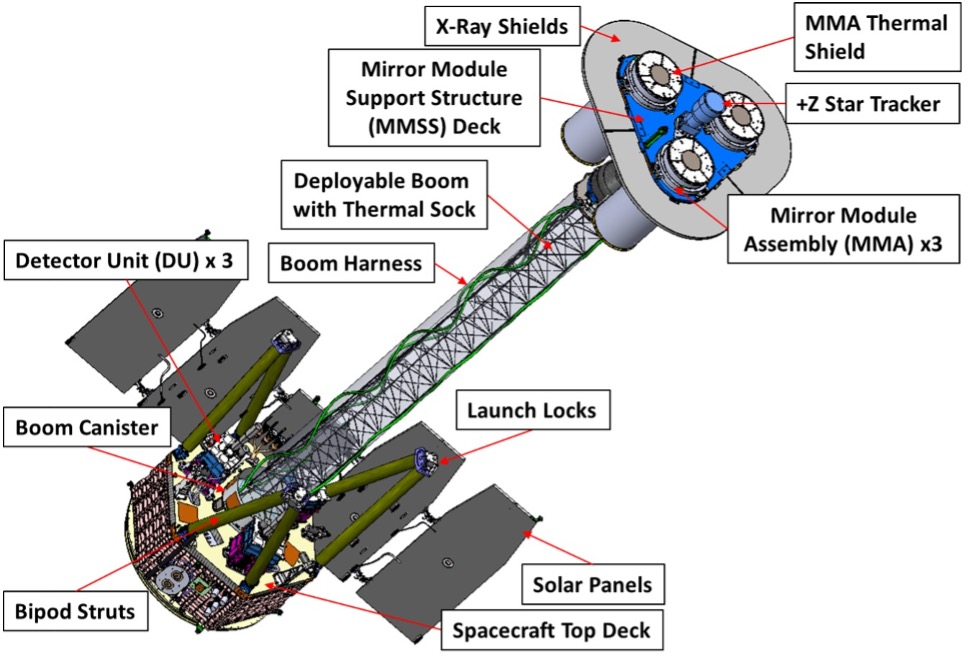
\includegraphics[width=0.6\linewidth]{figures/chapter3/ixpe}
    \caption{Schematic of the IXPE Observatory. Photons enter through the three Mirror Module Assemblies and are collcted by the Detector Units, where GPDs are located. Images courtesy of NASA.}
    \label{fig:ixpe}
\end{figure}

A detector unit (DU) is located on the focal plane of each telescope. A detector unit has a GPD to absorb and analyze X-ray photons, providing position, energy, timing and polarization information.


\section{Gas Pixel Detector}

At the basis of the operations of a GPD is the dependence of the photoelectron emission direction on the incident photon polarization, described by Eq. \ref{eq:polarization_photo}. Photons enter the active gas volume after passing through a beryllium window and can be absorbed. The primary ionization electrons produced by the photoelectron are drifted toward the GEM, which multiply the charges preserving the track shape. The charges generated after the multiplication stage are collected by the pixelated readout ASIC. A schematic example of the GPD and a track are shown in Fig. \ref{fig:gpd}.

\begin{figure}[!b]
    \centering
    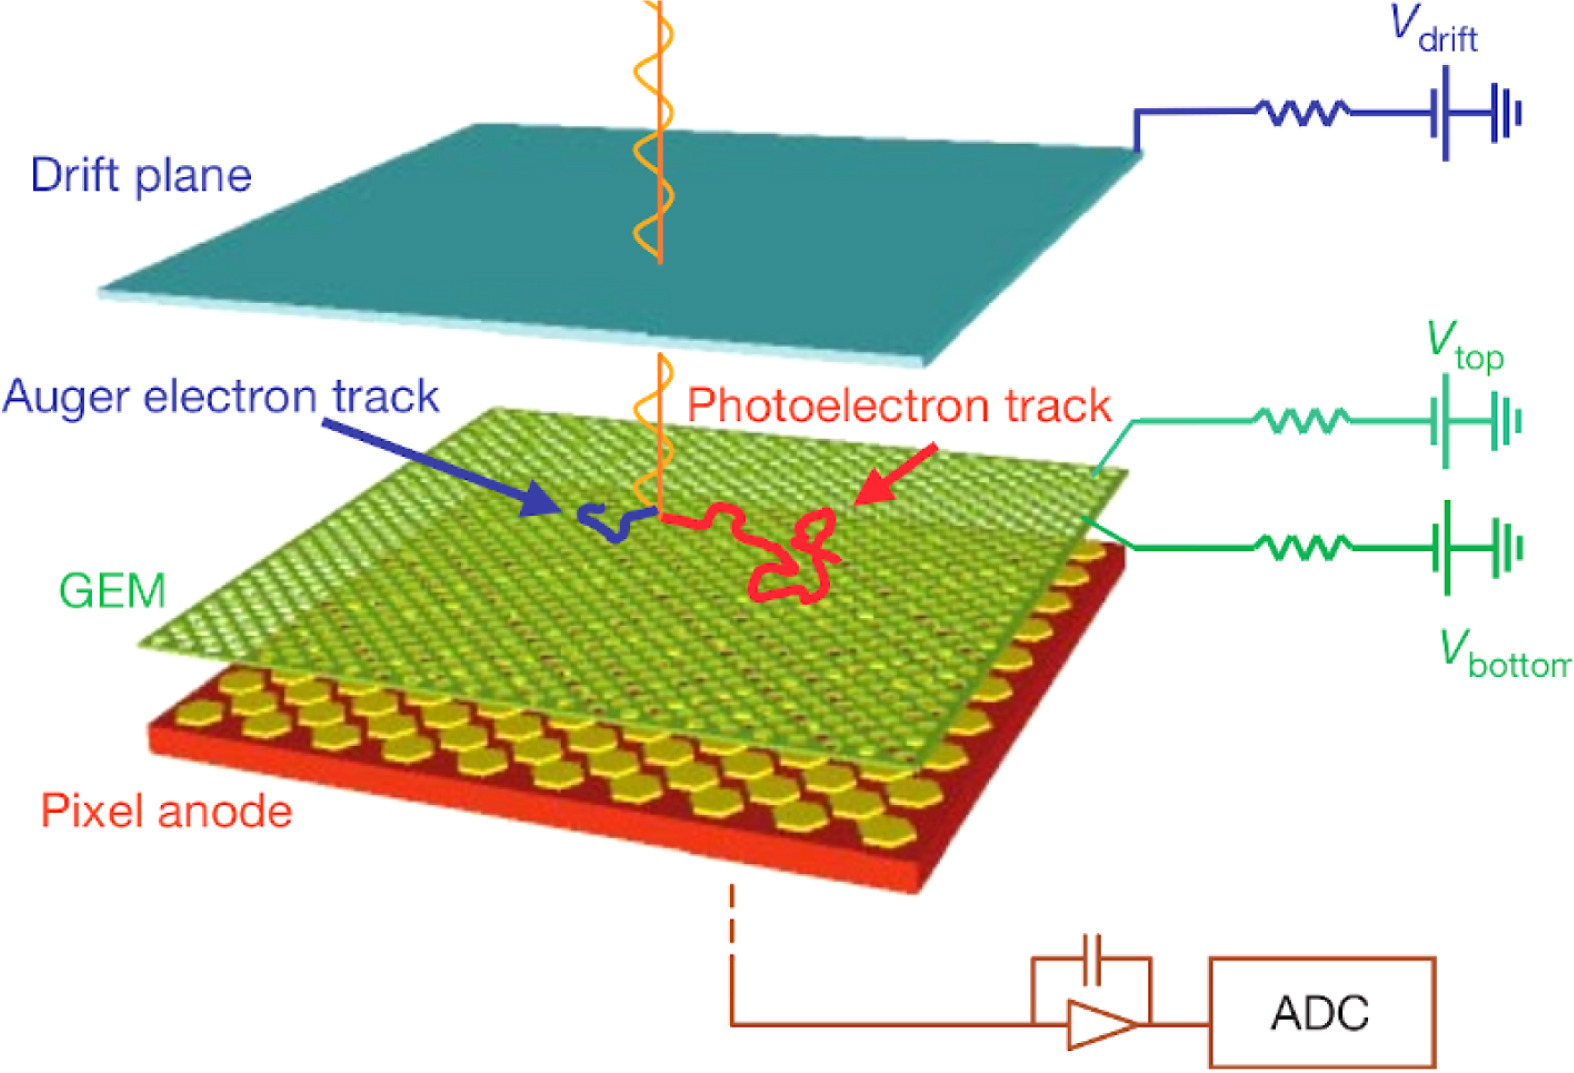
\includegraphics[width=0.49\linewidth]{figures/chapter3/gpd}
    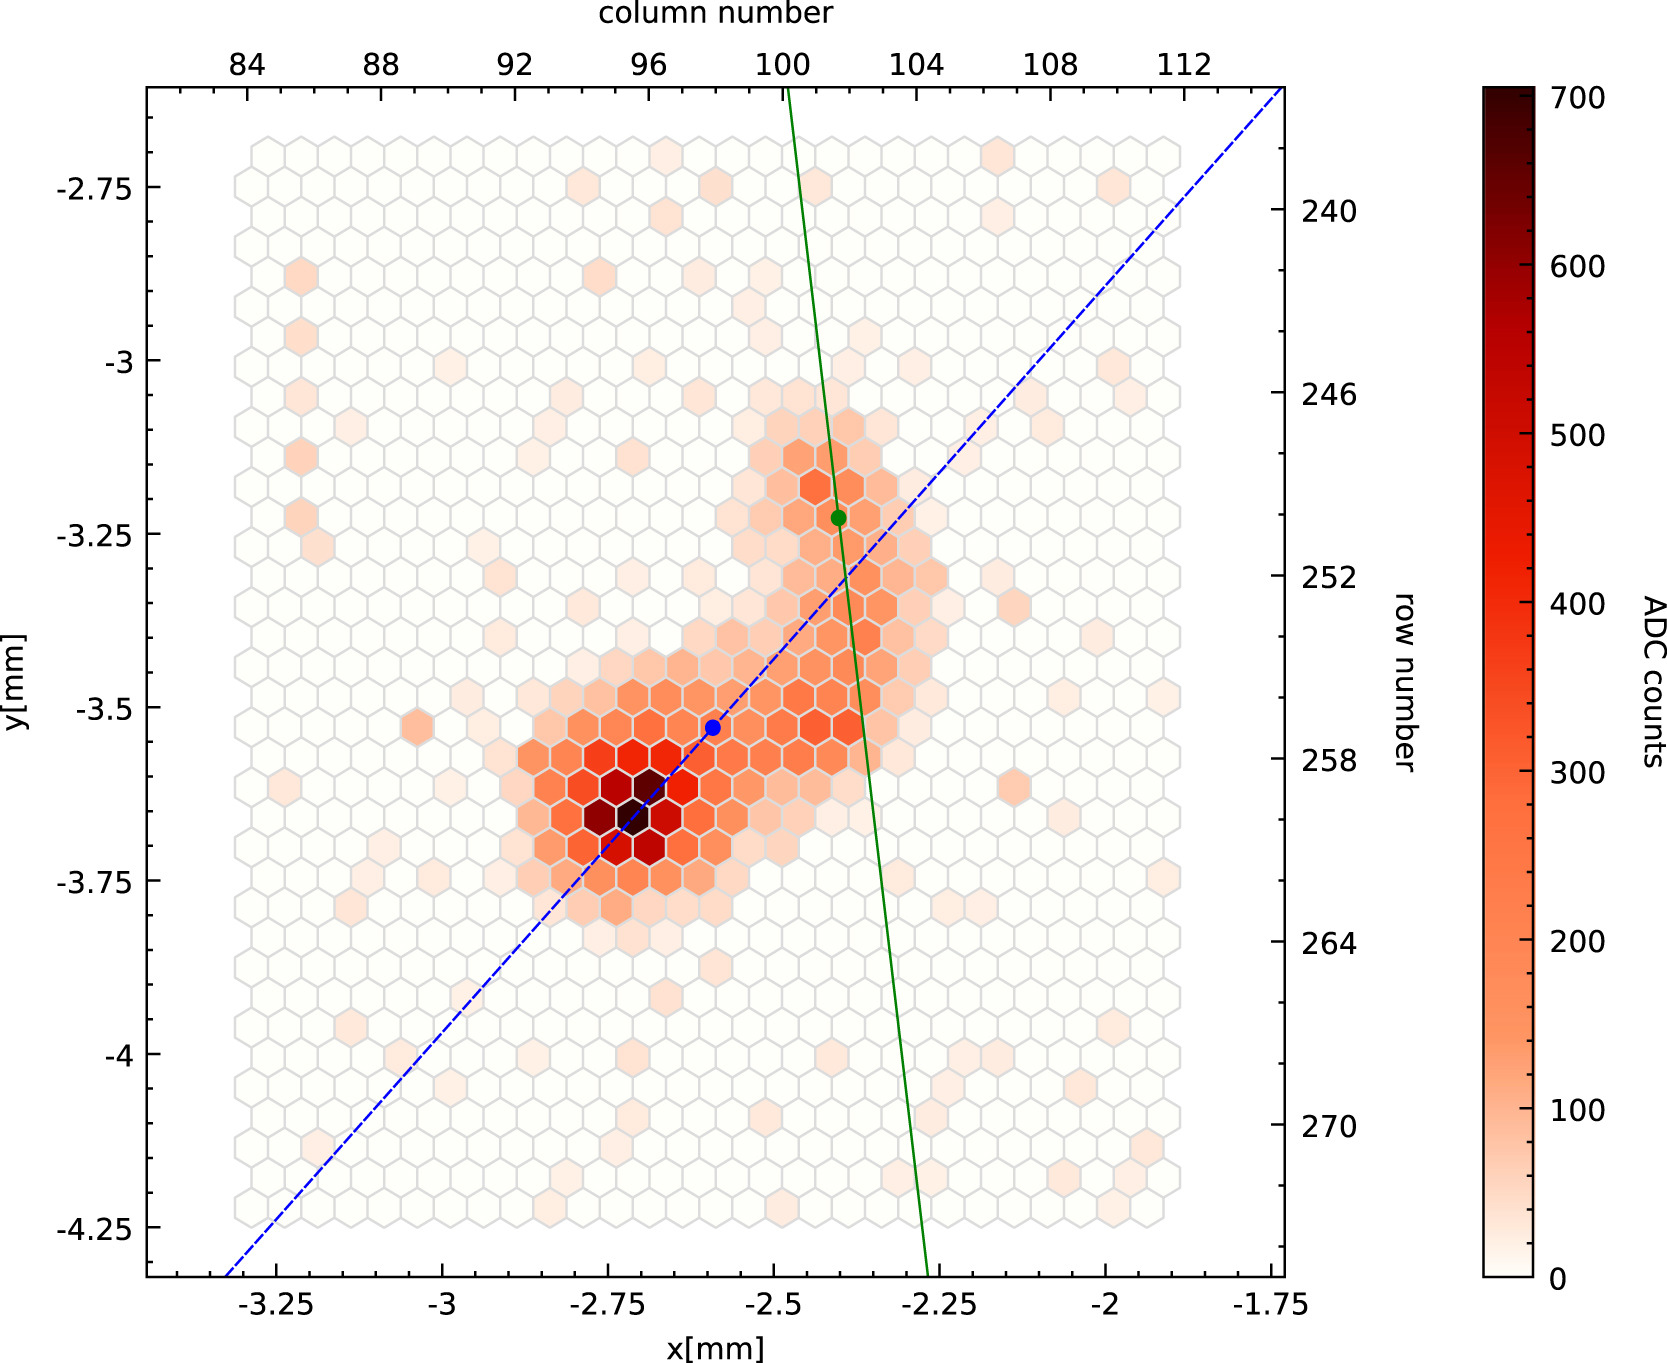
\includegraphics[width=0.49\linewidth]{figures/chapter3/track}
    \caption{The left panel shows the design of the GPD. A photon is aboserbed by the gas volume, producing a photoelectron which is drifted toward the GEM. The produced track is used to reconstruct the photoelectron emission direction. The signal is amplified by the GEM and is read with the dedicated pixelated readout ASIC. The right panel shows an example of a real track from a 5.9 keV photon. Images taken from \cite{baldini2021}.}
    \label{fig:gpd}
\end{figure}

\subsection{Gas cell}
The GPD active gas volume consists of pure dimethyl-ether (DME). The choice of using this gas was made because in order to work as a polarimeter it has to satisfy different requirements. The first is that a light-gas mixture enables to produce long and straight tracks, allowing for a higher efficiency in the polarization level estimate than what is achievable with high-$Z$ gas.

On the other hand, employing a gas mixture with low-$Z$ elements reduces the detector quantum efficiency.  However, there is another constraint which limits the maximum $Z$ that can be used, which is the $K$-edge energy. Indeed, the modulation described by Eq. \ref{eq:polarization_photo} holds only for absorption by spherical shells, thus it is fundamental that the $K$-edge energy is below the design sensitivity range of 2--8 keV.

DME therefore represents a good compromise to satisfy the design requirements. Furthermore, it is usually employed as a quencher, thus it is optimal to avoid accidental discharges in the detector that could compromise its functionalities.

A final important property of DME is that its transverse diffusion coefficient is low, about 68 $\mu$m cm$^{-\frac{1}{2}}$ with an electric field of 2 kV/cm, much lower than other typical gas mixtures (see Fig. \ref{fig:diffusion} for some examples), enabling to limit the track blurring, which represents a limiting factor in the reconstruction of the photoelectron emission direction.

\subsection{GEM}
The GEM \cite{sauli1997} represents the amplification stage of the GPD. A GEM usually consists of a 50 $\mu$m thick Kapton foil with a copper coating on both sides. The GEM is then etched to create holes, which can be tens of micrometers wide. A voltage difference is applied to the copper coatings on the two opposite faces of the GEM to generate a strong electric field inside the holes, as shown in Fig. \ref{fig:gem}.

\begin{figure}
    \centering
    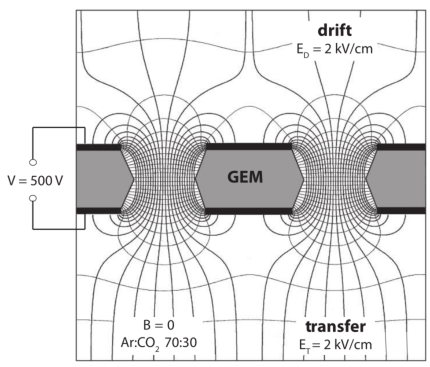
\includegraphics[width=0.49\linewidth]{figures/chapter3/gem_field}
    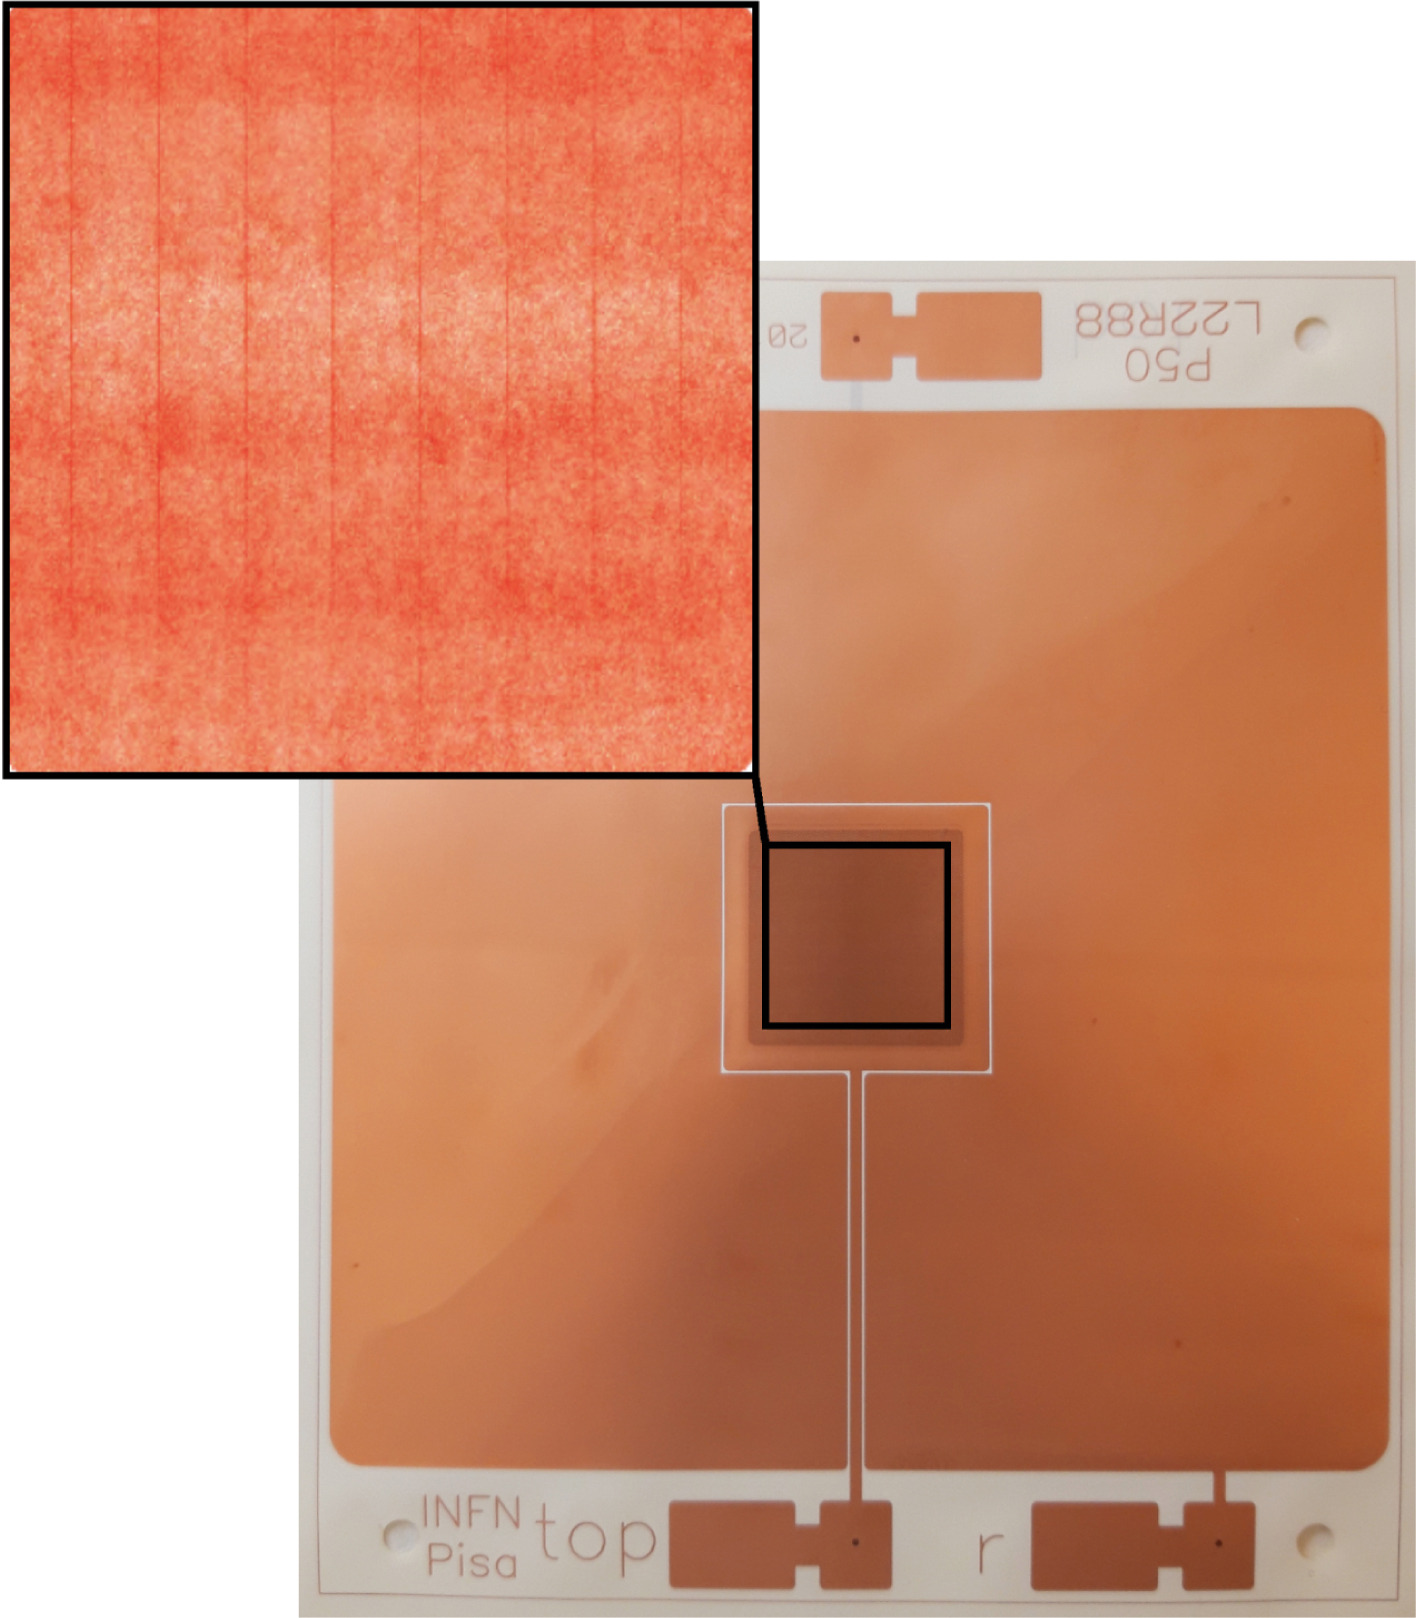
\includegraphics[width=0.4\linewidth]{figures/chapter3/gem}
    \caption{Electric field produced by GEM holes (left panel) when applying a voltage difference between the two copper electrodes (taken from \cite{kolanosky2020}). Photograph of a GPD GEM (right panel), with the darker region representing the active area of the GEM (taken from \cite{baldini2021}).}
    \label{fig:gem}
\end{figure}

The GEM employed inside the GPD is made of liquid crystal polymers (LPC) instead of Kapton, and holes have diameter of 30 $\mu$m. The hole pattern follows a hexagonal grid which matches the ASIC pixel pattern. The GPD GEM is shown in Fig. \ref{fig:gem}, and it is possible to observe the presence of eight equally spaced vertical lines. These lines are a result of the production process, which includes a step where the holes inside the LPC are made through laser drilling. The laser beam has a width smaller than the active region, and it needs multiple sweeps to complete the entire area.

The production process of the GEM directly affects the GPD performances. In particular, it introduces spatially dependent spurious modulations, as shown in Fig. \ref{fig:spurious_mod}. The real cause behind this systematic effect is not known, but one hypothesis is that GEM holes pitch can very along one direction.

In principle this systematic effect could be corrected by taking multiple acquisitions similar to that of Fig. \ref{fig:spurios_mod} by varying the source energy and for each GPD. However, the statistical accuracy required to correct this effect would have required to spend a prohibitive amount of time acquiring data for each detector. Instead of applying a direct correction, the solution adopted to mitigate this effect consists of exploiting the observatory dithering.

\begin{figure}
    \centering
    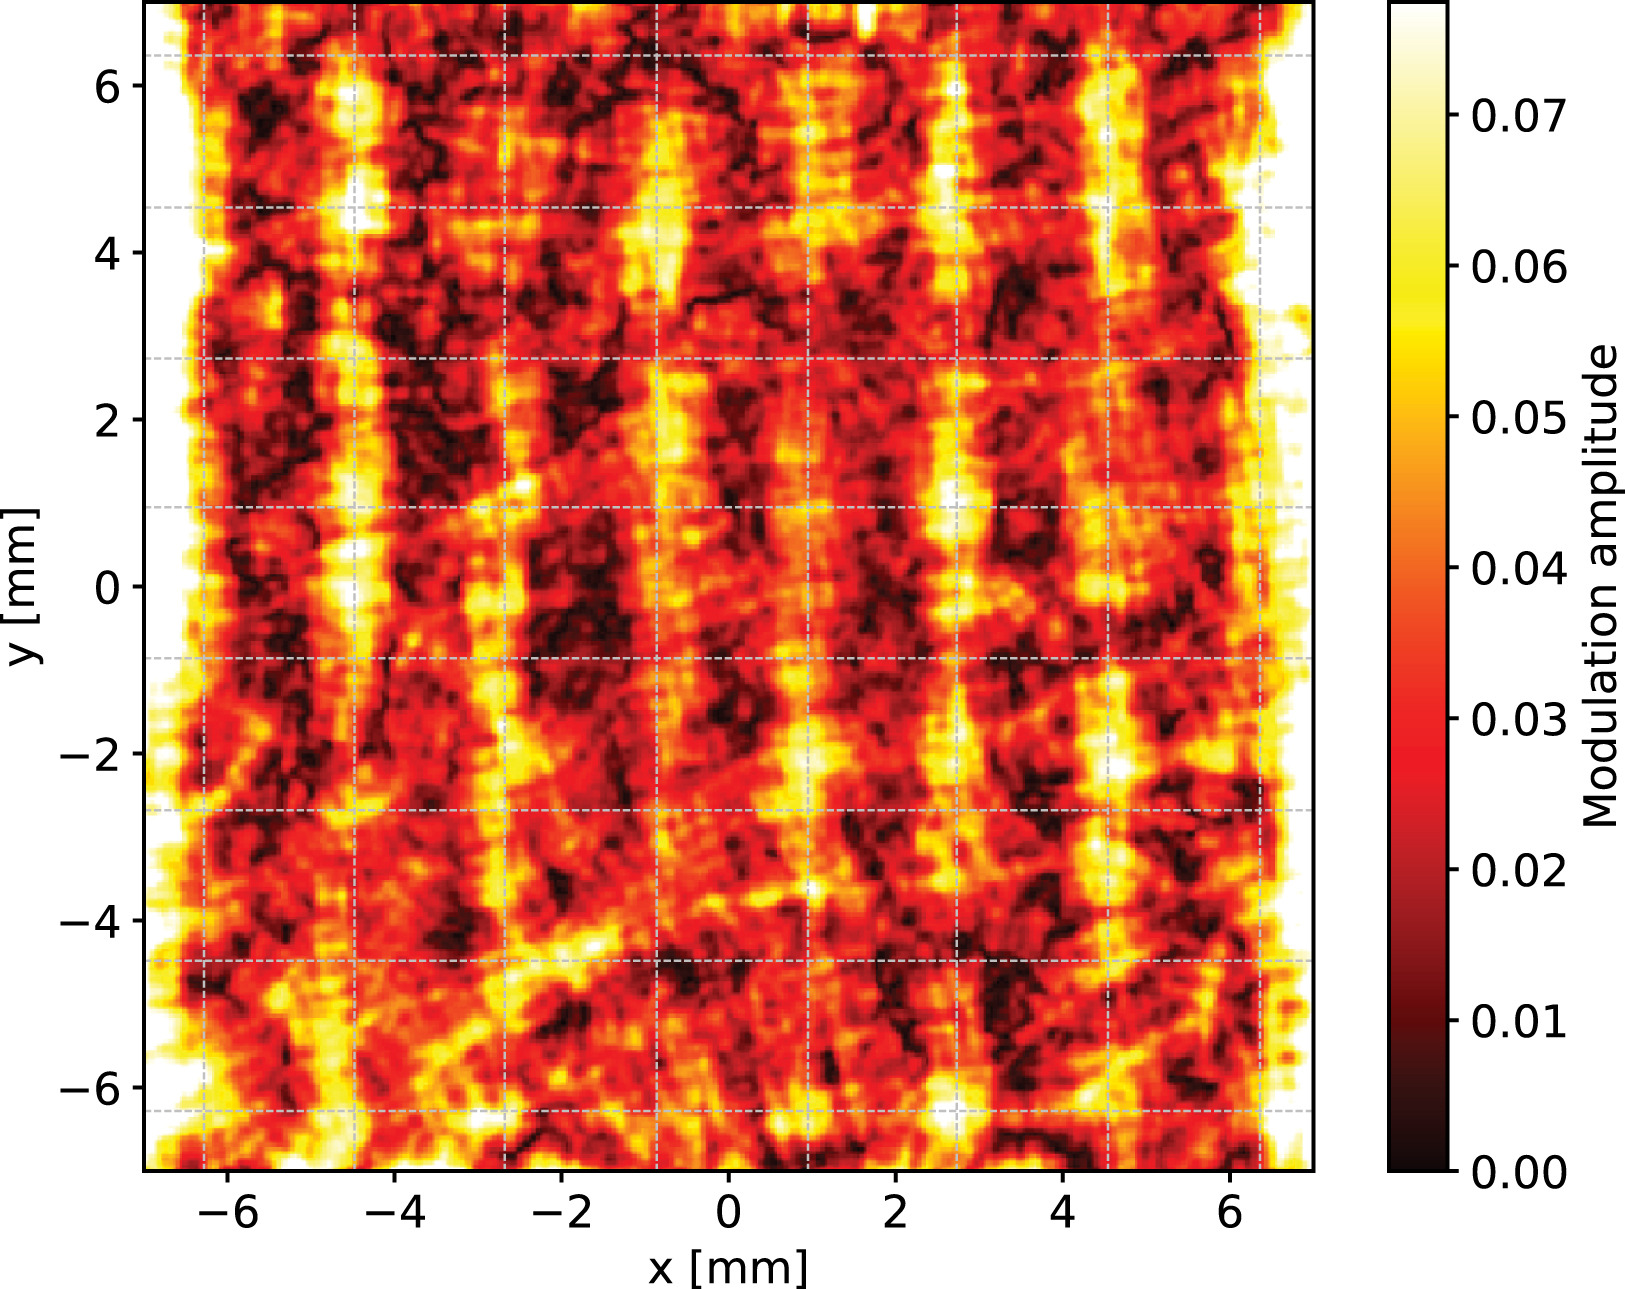
\includegraphics[width=0.49\linewidth]{figures/chapter3/spurious_mod}
    \caption{Modulation amplitude map obtained from an un-polarize X-ray source at 2.7 keV. The dashed gray grid correspond to the coordinates of the laser sweep overlaps (visible in Fig. \ref{fig:gem}) during the GEM production, and it perfectly overlaps with the regions with high-spurios modulation. Image taken from \cite{baldini2021}.}
    \label{fig:spurious_mod}
\end{figure}

Another important effect that depends on the GEM is rate-dependent gain variations. When the detector is operating and is irradiated by a source, part of the charge that is produced by the avalanche inside the GEM holes is temporarily deposited onto the dielectric substrate. This charging phenomenon has the effect of modifying the electric field configuration, with a consequent decrease of the gain.

When the detector is constantly illuminated by a fixed rate source, the gain does not decrease indefinitely but reaches a saturation level after which the gain is approximately constant. The asymptotic gain value and time scale of the process depend on the input energy flux.

This charging effect is reversible because the charge trapping on the dielectric substrate is not permanent. This phenomenon, which consists of a discharging of the dielectric, is a competing process of charging and is continuosly at play, but on much longer time scales. When the incoming flux is sufficiently low, discharging dominates over charging and the gain increases.

In general charging and discharging can be described as rate-dependent, and an example of these processes at play for GPD is shown in Fig. \ref{fig:rate_gain}.

\begin{figure}
    \centering
    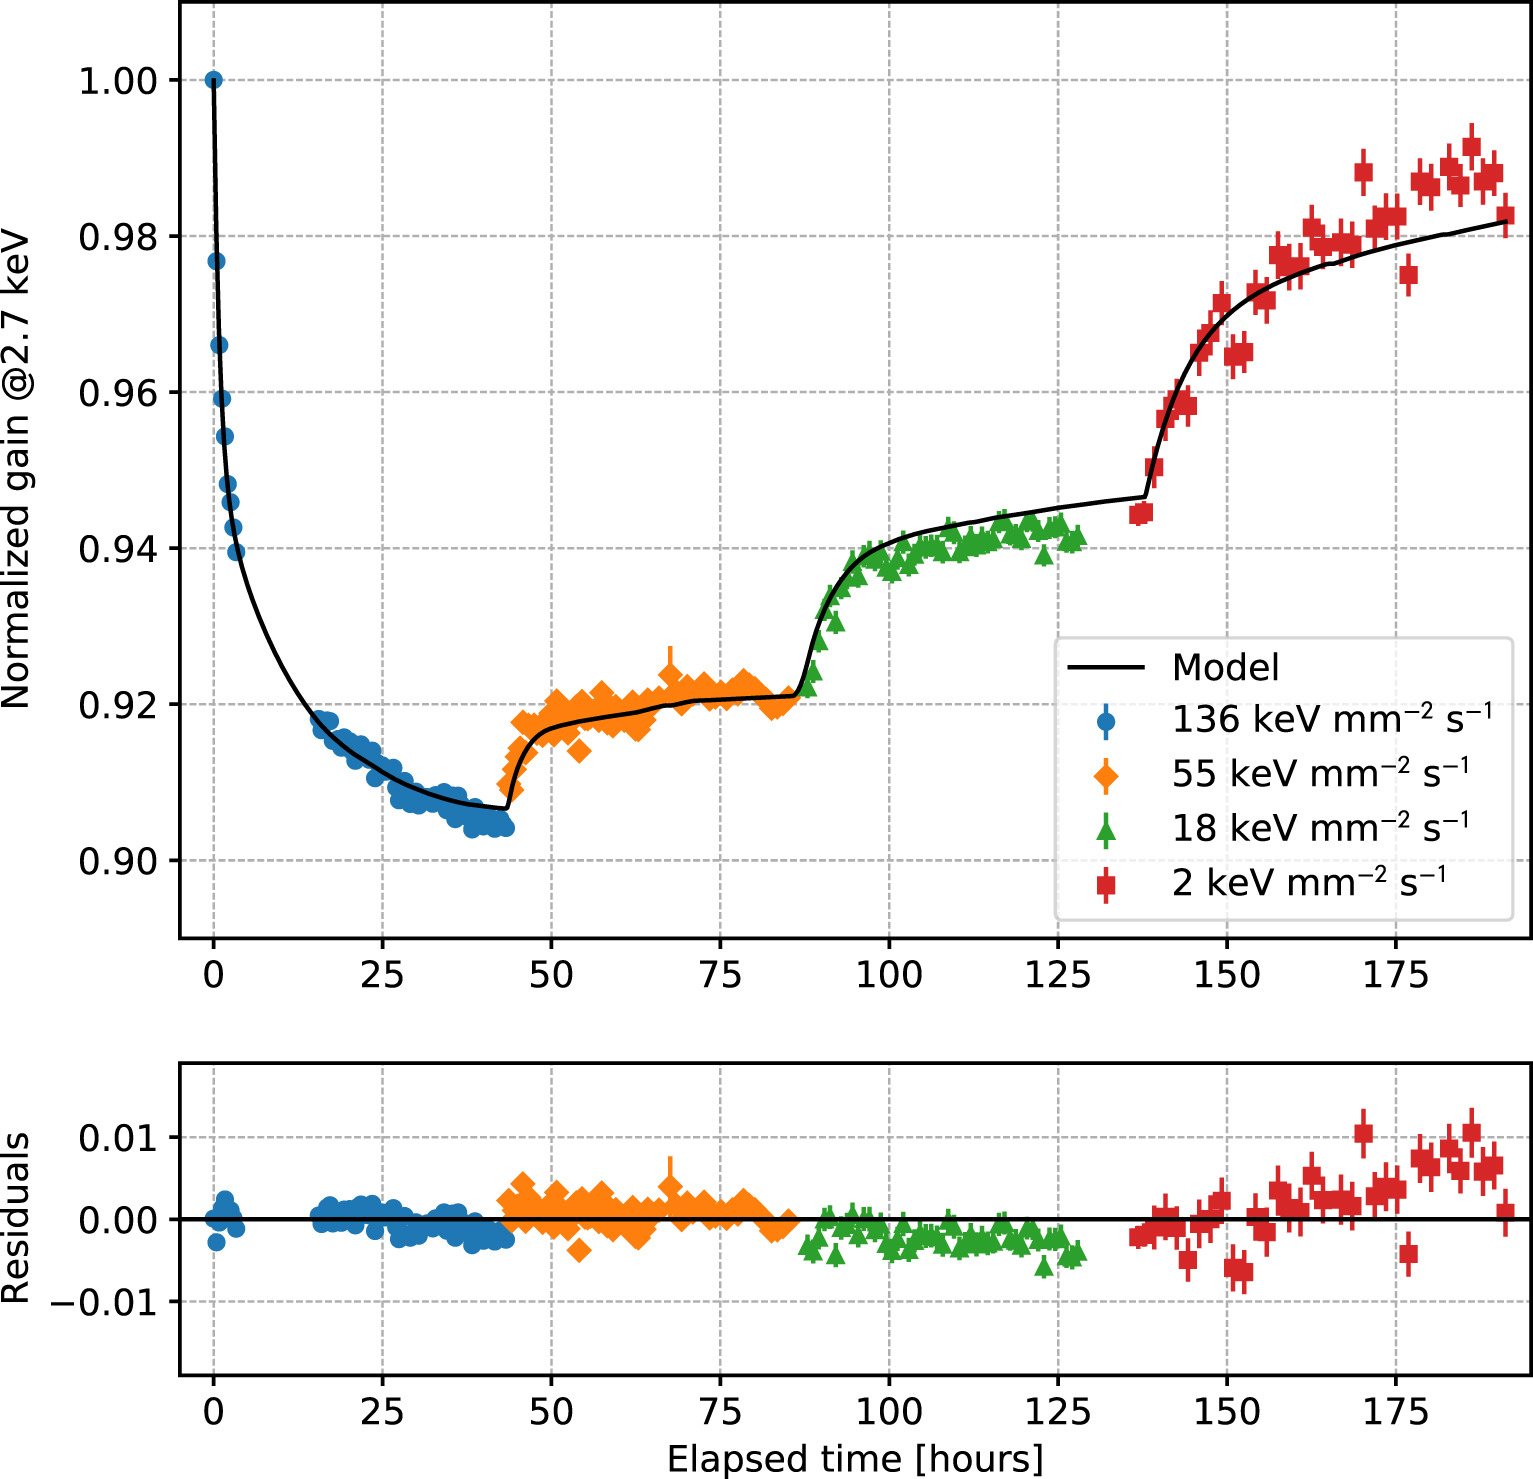
\includegraphics[width=0.49\linewidth]{figures/chapter3/rate_gain}
    \caption{Charging and discharging effects as a function of time for GPD. The different colors data points represent gain measurements taken with different input energy fluxes. First the charging is dominant with a high-flux source which causes almost 10\% of gain decrease. Then, the gain gradually recovers when using lower flux sources.}
    \label{fig:rate_gain}
\end{figure}

These gain variations can be modeled using phenomenological models and can be applied to correct observations. However, limiting the charging and reducing the gain variations amplitude can improve the detector sensitivity to polarization.

Reducing systematic effects, such as spurious modulation and gain variations, which have been observed with this type of GEM is the goal for the next generation of GPD, which is currently under study. One of the alternative which is being developed, which aims on reducing these effects, will be presented in Chap. \ref{chap:chapter5}.


\subsection{XPOL-I ASIC}

\cite{bellazzini2004, bellazzini2006}




\section{XPOL-III}


\label{sec:xpol3}
\cite{minuti2023}
